\documentclass[tikz,border=2pt]{standalone}
\usepackage{amsmath}
\usepackage{pgfplots}
\pgfplotsset{compat=1.18}
\usetikzlibrary{arrows.meta}
\begin{document}
% Density (1 - x/n)^(n-1) of the scaled uniform spacing n X_k^n on [0, n] for n = 2, 5, 20,
% approaching the Exp(1) density e^(-x); values at x = 1: 0.5, 0.41, 0.38 against e^(-1) = 0.37.
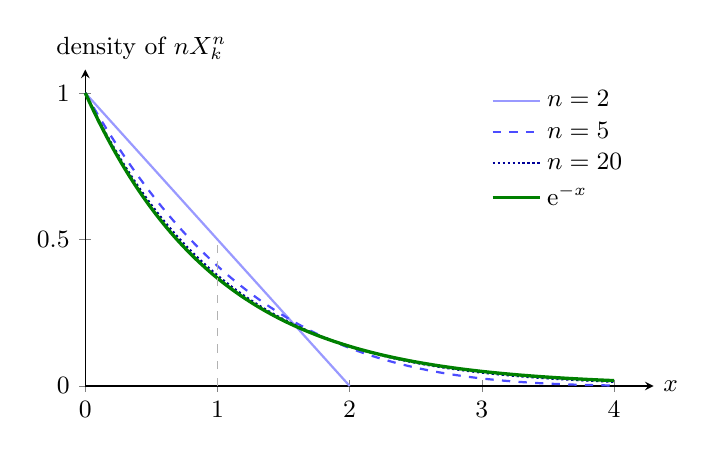
\begin{tikzpicture}[font=\small, >={Latex[length=2mm]}]
  \begin{axis}[
    axis lines=left, xmin=0, xmax=4.3, ymin=0, ymax=1.08,
    xtick={0,1,2,3,4}, ytick={0,0.5,1},
    xlabel={$x$}, ylabel={density of $nX_k^n$},
    xlabel style={at={(axis description cs:1,0)}, anchor=west},
    ylabel style={rotate=-90, at={(axis description cs:0,1)}, anchor=south west, xshift=-14pt},
    width=8.8cm, height=5.6cm, clip=false, samples=120,
    legend style={draw=none, fill=none, font=\small, at={(0.97,0.97)}, anchor=north east}, legend cell align=left
    ]
    \addplot[blue!40, thick, domain=0:2] {1-x/2};
    \addlegendentry{$n=2$}
    \addplot[blue!70, thick, dashed, domain=0:4] {(1-x/5)^4};
    \addlegendentry{$n=5$}
    \addplot[blue!60!black, thick, densely dotted, domain=0:4] {(1-x/20)^19};
    \addlegendentry{$n=20$}
    \addplot[green!50!black, very thick, domain=0:4] {exp(-x)};
    \addlegendentry{$\mathrm{e}^{-x}$}
    \draw[gray!60, thin, dashed] (axis cs:1,0) -- (axis cs:1,0.5);
  \end{axis}
\end{tikzpicture}
\end{document}
